\begin{frame} \frametitle{Testing approach (Training)}

	We trained the system registering 8 people:
	
	\begin{center}
 		\begin{tabular}{||c | c | c | c||} 
			 \hline
			 	\textbf{Real name} & 
			 	\textbf{id} & 
			 	\textbf{\#samples in gallery} & 
			 	\textbf{\#probes} 
			 \\ [0.5ex] 
			 \hline\hline
			 	Bill Gates & 
			 	bill & 
			 	60 & 
			 	10 
			 \\ 
			 \hline
			 	Barak Obama & 
			 	doubleb & 
			 	60 & 
			 	10 
			 \\
			 \hline
			 	Margot Robbie & 
				harley & 
			 	60 & 
			 	10 
			 \\
			 \hline
			 	Miriam Leone & 
			 	mlion & 
			 	60 & 
			 	10 
			 \\
			 \hline
			 	Scarlett Johansson & 
			 	redlucy & 
			 	60 & 
			 	10 
			\\
			 \hline
			 	Robert Downey Jr & 
				robman & 
			 	60 & 
			 	10 
			 \\
			 \hline
			 	Tom Hardy & 
			 	tommy & 
			 	60 & 
			 	10
			\\
			 \hline
			 	Mark Zuckerberg & 
			 	zuck & 
			 	60 & 
			 	10
			\\ [1ex] 
 			\hline
		\end{tabular}
	\end{center}	

\end{frame}

\begin{frame} \frametitle{Testing approach (Querying)}
	
	Then, we collected 10 other random pictures from the same 
	people, plus 10 pictures for other 5 people:
	
	\begin{itemize}
		\item Jimmy Fellon
		\item Donald Trump
		\item Tim Cook
		\item Jeff Bezos
		\item Alfred Hitchcock
	\end{itemize}
	
	To be quick, we used yet another script\footnote{This one: {\color{red} \url{https://git.io/JvsQv}}} to upload
	pictures to be queried. 
	
	\begin{block}{Use the script}
		./test /path/to/test-faces http://server.com /path/to/results.cvs
	\end{block}

\end{frame}

\begin{frame} \frametitle{Home-made gallery results (raw)}
	
	\begin{center}
		We let the script run and the results can be seen in this spreadsheet:
		\begin{figure}[H]
			
\includegraphics[width=.3\textwidth]{img/sheets}
		\end{figure}
		{\color{red} \url{https://tinyurl.com/rbk4dnc}}	
	\end{center}
	\vfill

\end{frame}

\begin{frame} \frametitle{Home-made gallery Results (Description)}

	We analyzed the results with a python script\footnote{{\color{red} 
	\url{https://git.io/Jvsp6}}}, and obtained these FAR and FRR:
	
	\vfill
	\begin{center}
		\begin{figure}[H]
			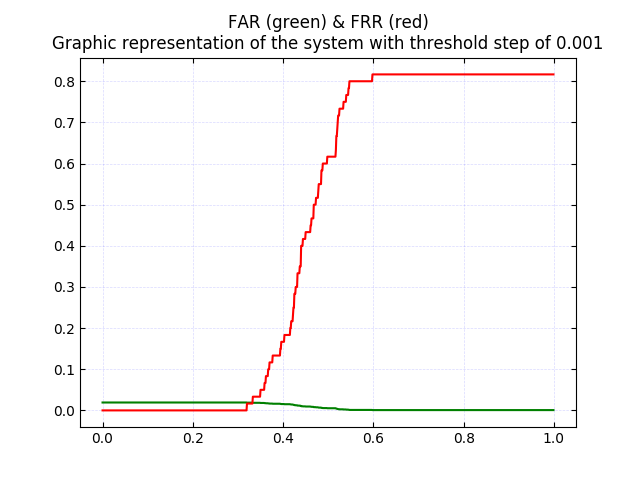
\includegraphics[width=.7\textwidth]{img/far-frr}
		\end{figure}
	\end{center}
	\vfill

\end{frame}

\begin{frame} \frametitle{LFW Results (raw)}

	\vfill
	We surely had more to test... That's why, instead of use our home-made 
	data set, we used the \textbf{Labeled Faces in the Wild}\footnote{
	{\color{red} \url{http://vis-www.cs.umass.edu/lfw/}}}. This time, 
	we used 75 registered users and 150 impostors, getting these results:
	
	\begin{center}
		\begin{figure}[H]
			
\includegraphics[width=.3\textwidth]{img/sheets}
		\end{figure}
		{\color{red} \url{https://tinyurl.com/skdethl}}	
	\end{center}
	\vfill

\end{frame}

\begin{frame} \frametitle{LFW gallery Results (Description)}

	We analyzed the results with a similar version of the precedent 
	python script\footnote{{\color{red} \url{https://git.io/JvGB8}}}, 
	and obtained these FAR and FRR:
	
	\vfill
	\begin{center}
		\begin{figure}[H]
			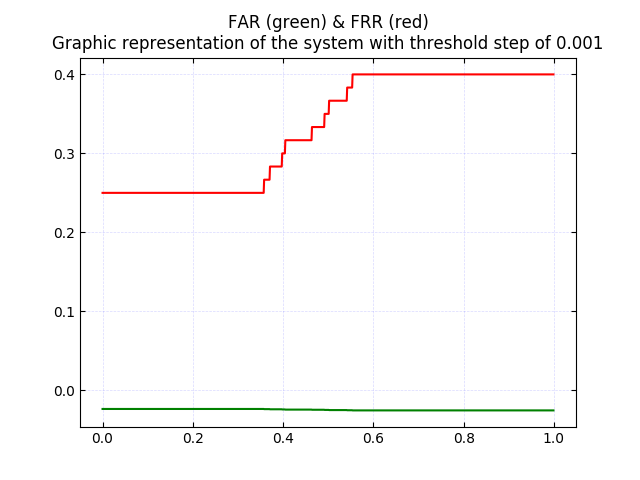
\includegraphics[width=.7\textwidth]{img/far-frr-lfw}
		\end{figure}
	\end{center}
	\vfill

\end{frame}
